%/////////////////////////////////////////////////////////////////////////////
%
% Definition des Dokuments
%
%/////////////////////////////////////////////////////////////////////////////
\documentclass[
11pt,				% Schriftgröße
a4paper,			% Seitengröße
DIV12,		     	% Satzspiegel
liststotoc,			% Inhalsverzeichnis in Inhaltsverzeichnis
bibliography=totoc, % Quellenverzeichnis in Inhaltsverzeichnis
listof=entryprefix, % Abbildungsverzeichnis in Inhaltsverzeichnis
listot=entryprefix, % Tabellenverzeichnis in Inhaltsverzeichnis
appendixprefix=true,
pointlessnumbers,
%	DIV=calc,		% Satzspiegel autom. berechnen, widerspricht sich mit vorherigem
%	twocolumn,		% Zweispaltiger Text
	oneside,		% Doppelseitig, während dem Arbeiten ausschalten, dann besser zum arbeiten, für digitale Variante auch ausschalten, 
%	BROC=10mm		% Bindeausgleich, Achtung links oder rechts anpassen
]{scrbook}

% Zeilenabstand
\usepackage{setspace}

% Absatzeinrückung und -abstand
\parindent 	= 0pt
\parskip 	= 6pt

% Dateicodierung
\usepackage[utf8]{inputenc} 

% Spracheinstellung
\usepackage[ngerman]{babel}
\usepackage[ngerman]{translator}

%Besondere Trennungen
\hyphenation{De-zi-mal-tren-nung}

% Zeichencodierung
\usepackage[T1]{fontenc}
\usepackage{titlesec}

% Schriften einstellen
\usepackage{lmodern}		%Vektorschrift, keine Pixel
\usepackage{microtype}		%Verbessert microtypographie, Verbessert auch warnings 	(overfull boxes)
\renewcommand{\familydefault}{\sfdefault} 	% {1}Standard Schrift, {2}entfernt Serifen, 													Schrift dann ähnlich Calibri
\usepackage{sansmath}		% Mathemodus ohne Serifen
%\sansmath					% Mathemodus aktivieren

\setcounter{secnumdepth}{3}
\setcounter{tocdepth}{3}

% Bilder einbinden
\usepackage{graphicx}
\usepackage{subfigure} 
\graphicspath{{Bilder/}}  % können mehrere Pfade eingebunden werden, von aktuellen Dokument ausgehend


% Dynamisch verlinktes Dokument
\usepackage[%pdfborder={0 0 0 }, 
colorlinks = true,
linkcolor = blue,
pdftitle={Titel der Abschlussarbeit},
pdfsubject={},
pdfauthor={Euer Name},
pdfkeywords={},	
]{hyperref}		%[]Art und Weise für die Anzeige


%------------- Literatur ------------------------------------
\bibliographystyle{unsrt}

\usepackage{color}
\definecolor{middlegray}{rgb}{0.5,0.5,0.5}
\definecolor{lightgray}{rgb}{0.8,0.8,0.8}
\definecolor{orange}{rgb}{0.8,0.3,0.3}
\definecolor{yac}{rgb}{0.6,0.6,0.1}
\usepackage{listings}
 \lstset{
	language=C++,
	basicstyle=\ttfamily,
	keywordstyle=\color{blue}\ttfamily,
	stringstyle=\color{red}\ttfamily,
	commentstyle=\color{green}\ttfamily,
	morecomment=[l][\color{blue}]{\#},
	backgroundcolor=\ttfamily\color{white},
	frame = single 
}

%--------------Große Tabellen---------------------------------------
\usepackage{longtable}
%------------------------Mathe----------------------------
\usepackage{amssymb}
\usepackage{nicefrac}
\usepackage{amsfonts}
\usepackage{amsmath}
%-----------------------------------------------------------


%Befehle von Klaus
\newcommand{\x}{\mathbf{x}}
\newcommand{\y}{\mathbf{y}}
\newcommand{\A}{\mathbf{A}}
\newcommand{\B}{\mathbf{B}}
\newcommand{\C}{\mathbf{C}}
\newcommand{\PP}{\mathbf{P}}
\newcommand{\tp}{^{\mathrm{T}}}
\newcommand{\mat}{\boldsymbol}
\newcommand{\xxi}{\boldsymbol{\xi}}

%------------- Definition der Titelseite ---------------------

\title{Implementierung eines Frameworks für generische Flugzeugsimulationen in C++}

\author{Abschlussbericht für das Modul Effizient Programmieren I \& II \\
	von \\
	Jan Olucak   }

%\label{
\publishers{durchgeführt am \\
	Institut für Aerodynamik und Gasdynamik \\
	der Universität Stuttgart \\
	[5ex]
	Stuttgart, im Juli 2018}

\date{}

% entweder erste Spalte fett oder Trennstrich, nicht beides

\usepackage{epsf}


%--------------- Kopf und Fusszeile --------------
\usepackage{scrpage2}
\pagestyle{scrheadings}
\clearscrheadfoot
\ifoot{}
\ofoot{\pagemark}

\automark[section]{chapter}
\ihead{\headmark}

\setheadsepline{0.2pt}

%\renewcommand{\thechapter}{\arabic{chapter}}
%\renewcommand{\thesection}{\arabic{section}}
%\usepackage{titlesec}
%------------------Hier beginnt das Dokument---------------------------------
%-----------------------------------------------------------------------------
%-----------------------------------------------------------------------------
\begin{document}
	
\maketitle							% fügt Titel in Dokument ein

\pagenumbering{Roman}
\pagestyle{empty}



\pagestyle{empty}
\tableofcontents
\newpage 
\pagestyle{scrheadings}
\setcounter{page}{1} 
\pagenumbering {Roman} 
\listoffigures
\newpage
\listoftables
\newpage

\renewcommand{\chapterpagestyle}{scrheadings}
\newpage
\include{Abbkuerzungsverzeichnis}
\newpage
\include{Symbolverzeichnis}

\pagestyle{scrheadings}
\setcounter{page}{1} 
\pagenumbering {arabic} 

% ab hier Zeilenabstand 1,5
\onehalfspacing
\renewcommand{\chapterpagestyle}{scrheadings}

\chapter{Einleitung}
\section{Ausgangslage}
\label{sec:ausgangslage}
Der Prozess des Flugzeugentwurfs erstreckt sich über mehrere Iterationen in denen das Flugzeug immer detaillierter ausgearbeitet wird. Um das Leistungsvermögen früh im Entwicklungsprozess zu beurteilen, können numerische Simulationen genutzt werden. Zum Einen werden mathematische Modelle benötigt, um das physikalische Verhalten von spezifischen Domänen des Flugzeuges abzubilden. Zum Anderen werden Parameter benötigt, um besagte Modelle zu beschreiben. Viele Parameter sind erst im Laufe des Entwurfsprozesses verfügbar. Um das Flugverhalten dennoch abzubilden, wird eine Simulation mit verschiedenen Ausbaustufen und Fehlermodellen benötigt.\\\\
In der Arbeit nach  \cite{Olucak.15.02.2017} wurde eine Matlab basierendes Programm entwickelt, mit dessen Hilfe Simulationsmodelle für Flugzeuge modelliert werden können. Die fertigen Modelle werden sowohl in Text-Files, als auch komprimierten mat-files gespeichert. Um die Modelle zu validieren wurde zudem eine Simulation mit 6 Freiheitsgraden implementiert. Das Programm Aircraft Designer kann jederzeit um weitere Methoden ergänzt werden, um so den Entwurfsprozess fortzusetzen. Mittels dem semi-empirischen Tool DataCompendium (DATCOM) wird die Aerodynamik des Flugzeuges für zuvor definierte Flugzustände berechnet. In einem automatisierten Prozess wird ein Vorgaberegler für die Flugzustände entworfen. Ist der Entwurfsprozess abgeschlossen kann durch die zuvor erwähnte Simulation die Güte der Modelle beurteilt werden und gegebenenfalls durch Anpassung der Parameter modifiziert werden. Die Laufzeit ist mitunter eine sehr kritische Größe. Zudem ist eine objektorientierte Programmierung nur bedingt möglich, was den Ausbau zu einer generischen Simulation erschwert.
\newpage
\section{Zielsetzung}
Innerhalb dieser Ausarbeitung soll eine generische Flugzeugsimulation in der Hochsprache C++ implementiert werden. Generisch bedeutet in diesem Zusammenhang, dass die Simulationsumgebung nicht auf einen spezifischen Entwurf bezogen ist, sondern verschiedene Entwürfe mit dem in \cite{Olucak.15.02.2017} entstandenen Aircraft Designer simulierbar sind. Somit sollen die Methoden sehr allgemein gehalten werden.  Jede Ausbaustufe des Entwurfsprozesses soll simulierbar sein, ohne dass dabei der Code verändert wird. Über Input-Files sollen verschiedene Domänen-Modelle ausgewählt und die Simulation gesteuert werden können.  Ein modularer Aufbau soll zudem eine einfache Erweiterung des Simulation gewährleisten. Zudem soll die Performance der Simulation hinsichtlich Rechenzeit gegenüber Matlab verbesert und im Nachgang weiter optimiert werden. Um das Simulations-Framework zu validieren, wird die in \cite{Olucak.15.02.2017} implementierte Simulation in C++ übersetzt. Der gesamte Entwicklungsprozess stützt sich dabei auf die in \cite{Kessler.Sommersemester2017} vorgestellten Methoden und Anregungen.
 


\chapter{Aufbau der Simulation}
\section{Grundidee des Simulation-Frameworks}
Für die Umsetzung einer generischen Simulation werden die einzelnen Domänen des Flugzeuges in Modulen implementiert. Innerhalb der Module werden die verschiedenen Ausbaustufen oder mathematischen Modelle der Domänen implementiert. Um nun einen generischen Aufruf zu gewährleisten wird eine Klasse gleichnamig zu dem jeweiligen Modul implementiert, in der zum Einen die Auswahl für das jeweilige Modell getroffen wird, zum Anderen der eigentlichen Funktionsaufruf. Die Auswahl wird über ein Input File durch Veränderung eines Parameters getroffen. \\
Um nun einen generischen Aufruf zu gewährleisten wird in jedem Modul einen Basis-Klasse definiert. Neue Modelle können von der Basis-Klasse selbst oder von einem Kind der Basis-Klasse erben. Wird nun über das Input-File ein Modell ausgewählt, wird über eine switch-Funktion die Basis-Klasse initialisiert, wobei der Zeiger auf das jeweilige Modell gerichtet wird. \\
\begin{figure}[h]
\centering\includegraphics[width=0.3\linewidth]{UML_modul.PNG}	
\caption{UML Diagramm des grundlegenden Funktionsaufruf}
\label{fig:UML_modul}
\end{figure}

Somit kann das Modul jederzeit um neue Modelle erweitert werden, ohne den Funktionsaufruf selbst anzupassen.  
\section{Ablauf der Simulation}

\section{Ausbaustufen der Simulation}


\chapter{Durchführung der Implementierung}
\section{Implementierungs-Prozess}
Für die Validierung des Frameworks wird die Matlab-Simulation nach \cite{Olucak.15.02.2017} verwendet. Da es hier lediglich um eine Konvertierung des Codes handelt, werden die mathematischen Modelle nicht explizit erklärt. Vielmehr wird das Vorgehen der Implementierung erläutert, um zu zeigen, wie das Programm effizient entwickelt wurde. Gleiches gilt für die Implementierung der Simulationswerkzeuge.\\
 Die Simulations-Umgebung wurde sukzessive aufgebaut. Es wurde stets darauf geachtet, dass nach der Implementierung einer Funktion nach Möglichkeit direkt getestet wurde. Erst mit der nachgewiesenen Funktionalität, wurde der nächste Schritt im Prozess durchgeführt, wie In Abbildung \ref{fig: ImpProzess} dargestellt.
\begin{figure}[h]
	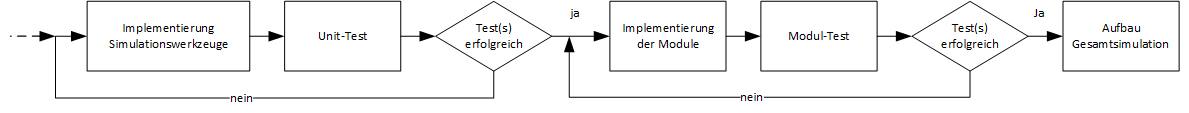
\includegraphics[width=1.0\linewidth]{ImpProzess.PNG}
	\caption{Flussdiagramm des Implementierungs-Prozess}
	\label{fig: ImpProzess}
\end{figure}
\section{Simulationswerkzeuge}
Unter Simulationswerkzeugen sind Funktionen zu verstehen, die in allen Teilen des Simulations-Frameworks vorkommen. Dies umfasst beispielsweise das Einlesen und Schreiben von Simulationsparametern oder mathematische Funktionen wie Integration oder Interpolation. Es ist offensichtlich, dass besagte Funktionen als erstes implementiert werden müssen, damit die Module im späteren Verlauf auf diese zurückgreifen können. Diese Werkzeuge wurden eigens in das Modul \textbf{Tools} implementiert. Auch die in \ref{sec:OSBib} beschriebenen Bibliotheken fallen unter diese Werkzeuge. Die implementierten Simulationswerkzeuge werden in Tabelle \ref{tab: SimWerk} zusammengefasst.
\begin{table}[h]
\centering	\begin{tabular}{lp{11cm}}
		\textbf{Funktion/Klasse} & \textbf{Kurzbeschreibung}\\
		 Constants & physikalische Konstanten\\\\
		 DataLogger & Erzeugung von Text-Files (Output der Simulation)\\\\
		 LinearInterpolation & Ein- und zweidimensionale Interpolation \\\\
		 MatFileReader & Funktionen zum Einlesen von .mat-File\\\\
		 ODESolver & Template(s) für numerische Integration\\\\
		 readInData & Funktionen zum Einlesen von Parametern aus Text-Files\\\\
		 Transformation & Matrizen für Koordinatentransformation
	\end{tabular}
\caption{Simulationswerkzeuge der generischen Flugzeugsimulation}
\label{tab: SimWerk}
\end{table}
\newpage
\subsection{Unit-Tests}
Um sicherzustellen, dass die Werkzeuge korrekt implementiert wurden, wurden Unit-Test definiert. Dazu wurde das von Visual Studio bereitgestellte Microsoft-Komponententest-Frameworks für C++ genutzt, um die Tests manuell durchzuführen. Die Unit-Tests wurden in einen gleichnamigen Projektordner ausgelagert. An dieser Stelle werden nicht alle Test erklärt. Vielmehr soll das Test-Schema erläutert werden. In dieser Arbeit wird das AAA-Schema  (Arrange, Act, Assert) nach \cite{Microsoft.2018}  genutzt. Dazu werden die Tests in die zuvor genannten Abschnitte aufgeteilt. Im einzelnen haben die Abschnitte folgende Bedeutung \cite{Microsoft.2018}: 
\begin{itemize}
	\item  \underline{Arrange} dient der Initialisierung des Tests. Die benötigten Objekte werden initalisiert und Parameter für den Testfall festgelegt.   
	
	\item  Innerhalb von \underline{Act} wird die zu testende Methode mit den zuvor definierten Testfall/Parametern aufgerufen.
	
	\item Im Abschnitt \underline{Assert} werden die Referenzwerte mit den Werten aus dem eigentlichen Test vergleichen. Wird eine Übereinstimmung festgestellt, erhählt der Testfall seine Bestätigung durch das Framework.
\end{itemize}
Die Referenzwerte wurden entweder selbst festgelegt (z.B. Einlesen eines Parameters) oder es wurde Matlab genutzt, um Referenzwerte zu generieren (z.B. Interpolation). \\
Nach \cite{TuxFamily.2018} handelt es sich bei \textbf{eigen} um eine vollständig getestete Bibliothek. Aus diesem Grund wurden nur Unit-Tests für einige wichtige Funktionen durchgeführt. Bei der auf \cite{Hulbert.2013} beruhenden MatFileReader-Klasse wird nur der selbst geschrieben Code getestet. Eine Außnahme bei den Unit-Test stellt das Header-File Constants, bei der lediglich physikalische und mathematische Konstanten hinterlegt sind. 

\section{Implementierung und Testen der Module}
In Abschnitt \ref{sec:AufbauModule} wurde bereits der Aufbau der Module erläutert und in Tabelle \ref{sec:Ausbaustufen} die für die Simulation benötigten Module aufgelistet. Um deren Funktionalität nachzuweisen, wurden Modul-Tests durchgeführt. Wie schon erwähnt, wird die 6 Dof-Simulation nach \cite{Olucak.15.02.2017} genutzt, um das Simulations-Framework zu testen. Somit liegen nur zu den dort verwendeten Modellen Referenzwerte vor. In diesem Abschnitt beziehen sich die Tests nicht auf das jeweilige Gesamtmodul, sondern lediglich auf die bisher implementierten Klassen.
Die Schwierigkeit, die mit den Modul-Tests einhergeht, ist die Definition der Testfälle. Ziel ist es eine größtmögliche Testabdeckung zu haben, um zu garantieren, dass das Modul wie gewünscht funktioniert. Bei einigen Modulen ist das Testen nur bedingt oder  nur im Gesamtsystem-Test möglich. Dies betrifft beispielweise das \textbf{Autopilot} und \textbf{Guidance} Modul. Für beide Module werden Parameter von anderen Modulen benötigt. \\Eine weitere Problematik besteht bei den verschiedenen  Modellen der Ausbaustufen.  Für die Simulation mit 3 Freiheitsgraden liegt keine Referenz vor. Ähnlich verhält sich die 6 Dof-Simulation mit Fehlermodellen. Es liegen aktuell keine Modelle für Sensorik und Aktuatorik vor. Somit können an dieser Stelle keine Modul-Tests für die zusätzlichen Module erfolgen.
In Tabelle \ref{tab:modultests} werden die Module  und deren Testfälle aufgezeigt, für die ein Modul-Test in Betracht kommt.\\
\begin{table}[h]
\centering	\begin{tabular}{l p{12cm}}
		\textbf{Modul} & \textbf{Beschreibung Testfall}\\
		Atmosphere & Bei dem hier hinterlegten Modell  handelt es sich um die US Standard-Atmosphäre von 1976.  Temperatur, Druck, Dichte und Schallgeschwindigkeit sind hierbei abhängig von der Flughöhe. Somit werden die zuvor beschriebenen Größen von 0-10000m berechnet und mit Daten der Standard-Atmosphäre verglichen.\\\\
		Aerodynamic & Hier wird ein Windtunnel bei konstanter Höhe simuliert. Es werden Machzahl, Anstellwinkel und Höhenruder-Winkel variiert. Es ist ersichtlich, dass nur die Längsbewegung betrachtet wird. Dies ist auf mangelnde Referenzwerte für die Seitenbewegung zurückzuführen. Ziel dieses Tests ist es die Polare des Flugzeuges abzufahren und mit den Matlab-Daten zu vergleichen. \\\\
		Guidance &  Es wird lediglich getestet, dass für den jeweiligen Zeitschritt die richtige Soll-Querbeschleunigung vorliegt. Das Modul selbst kann erst im Gesamtsystemtest vollständig getestet werden, da die jeweiligen Flugzustände benötigt werden.\\\\
		Trajectory & Der Trajectory-Modul Test testet die korrekte Berechnung der Flugbahn. Hier wird die Matlab-Simulation simuliert. Im Anschluss können die Ergebnisse verglichen werden.
	\end{tabular}
\caption{Auflistung der Modultests}
\label{tab:modultests}
\end{table}
\newpage
Aufgrund der Einfachheit des aktuell hinterlegten Schub-Models (Engine-Modul) wurde auf einen Modul-Test verzichtet und der Nachweis über Code-Reading durchgeführt.
Es ist offensichtlich, dass das Trajektorien-Modul erst aufgebaut werden konnte, nachdem die dafür benötigten Module bereits erfolgreich getestet wurden. Die Überprüfung der Tests erfolgte rein qualitativ und die Ergebnisse der Unit- und Modultests wurde im Ordner \textbf{Test Results} hinterlegt.


\section{Validierung des Simulations-Framework}
Abschluss des Implementierung stellt der Gesamtsystemtest des Simulations-Framework. Dazu wird das \textbf{Aircraft} Modul mit den Simulationsparametern nach \cite{Olucak.15.02.2017} initialisiert.\\
Ziel von \cite{Olucak.15.02.2017} war es, den Flugzustandsregler zu testen. Dem Vorgaberegler wurden Querbeschleunigungen für jeden Zeitschritt als Soll-Wert vorgegeben. Ziel war es, dass das Flugzeug den Querbeschleunigungen folgt.\\ In Abbildung \ref{fig:valSim} sieht man, wie der Ist-Wert des Reglers den Soll-Werten der Guidance  sehr gut folgt. Die anfänglichen Schwingungen sind auf die Initialisierung der Simulation am Trimmpunkt zurückzuführen. Da die Arbeitspunkte durch Linearisierung gefunden werden, entsteht ein Modellfehler.
\begin{figure}[h]
	\centering
	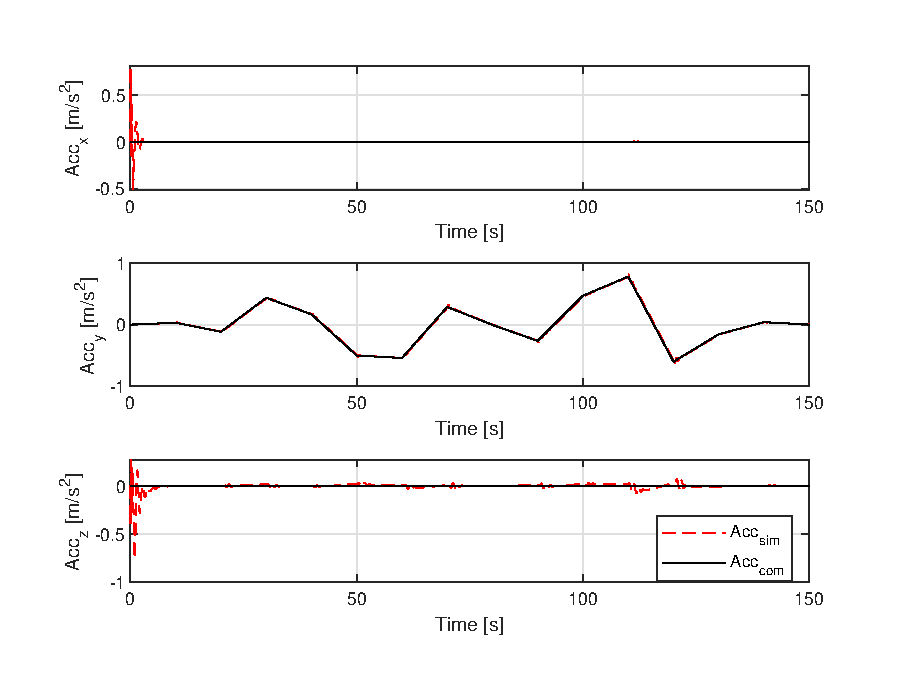
\includegraphics[width=0.7\linewidth]{querbeschleunigungen}
	\caption{Validierung der Simulation}
	\label{fig:valSim}
\end{figure}\noindent\\
Da kein Bahnregler implementiert wurde, ist es weniger zielführend die Trajektorie selbst zu betrachten. Weitere Simulationsergebnisse sind im Anhang unter \ref{sec:simerg} dargestellt.
Nachfolgend werden die Ergebnisse von Matlab und C++ verglichen.
 \newpage
 \begin{minipage}{0.49\linewidth} 	
 		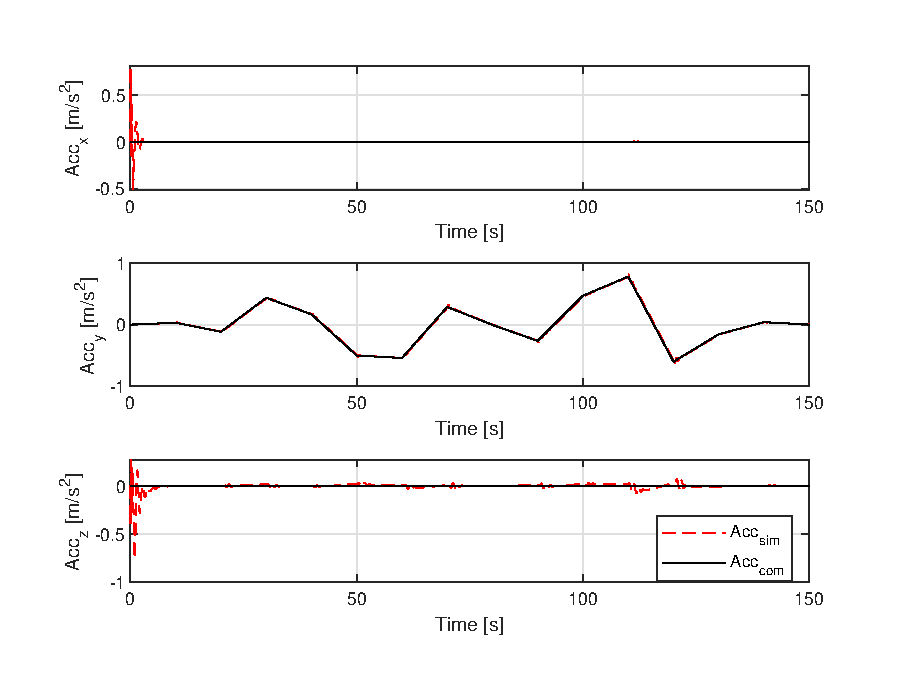
\includegraphics[width=1.0\linewidth]{querbeschleunigungen}
 \end{minipage}
 \begin{minipage}{0.01\linewidth}
	\hfill
\end{minipage}
 \begin{minipage}{0.49\linewidth}
		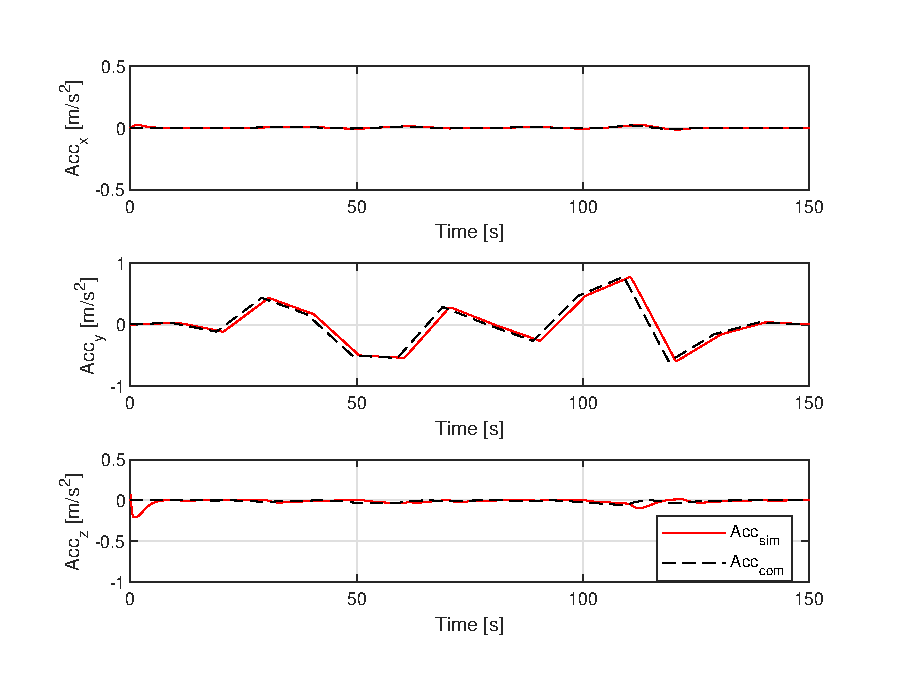
\includegraphics[width=1.0\linewidth]{matSim}
\end{minipage}
\captionof{figure}{Vergleich der Simulationsergebnisse, links C++, rechts Matlab}\noindent\\
Bei beiden Simulationen sind die Initialisierungsfehler zu erkennen, wobei in C++ die anfänglichen Schwingungen größere Amplituden besitzen. Offensichtlich folgt die Simulation in C++ der Soll-Werten besser als in Matlab. Zudem sind auch numerische Unterschiede zu erkennen. In \cite{Unbekannt.2012} und \cite{Unbekannt.2011} wurden diese numerischen Unterschied zwischen Matlab und C/C++ diskutiert. Beruhend auf diesen Quellen ist es zu erwarten, dass die beiden Ergebnisse nicht vollständig übereinstimmen und die Berechnung in C++ genauer ist. Die Simulation nach \cite{Olucak.15.02.2017} diente nur der Validierung und nicht der Verifikation. Das Ziel, dass das Flugzeug den Querbeschleunigungsvorgaben folgt, wurde erfüllt. Die Ausbaustufe mit 6 Freiheitsgraden konnte somit validiert werden.\\ Die höchste Ausbaustufe liefert die gleichen Ergebnisse wie die Ausbaustufe ohne Fehlermodelle. Wie in \ref{sec:Ausbaustufen} beschrieben, sind nur Methoden implementiert, die ein fehlerfreies Verhalten simulieren. Somit konnte auch diese Ausbaustufe erfolgreich getestet werden. Auf eine Visualisierung wurde an dieser Stelle verzichtet.
\newpage
\subsection{Direktvergleich Rechenzeit Matlab und C++}
In Abbildung \ref{fig:direktvergleich} wird die Rechenzeit der Simulation in Matlab und C++ gegenübergestellt. Der Performance Gewinn in C++ ist offensichtlich zu erkennen.
\begin{figure}[h]
	\centering
	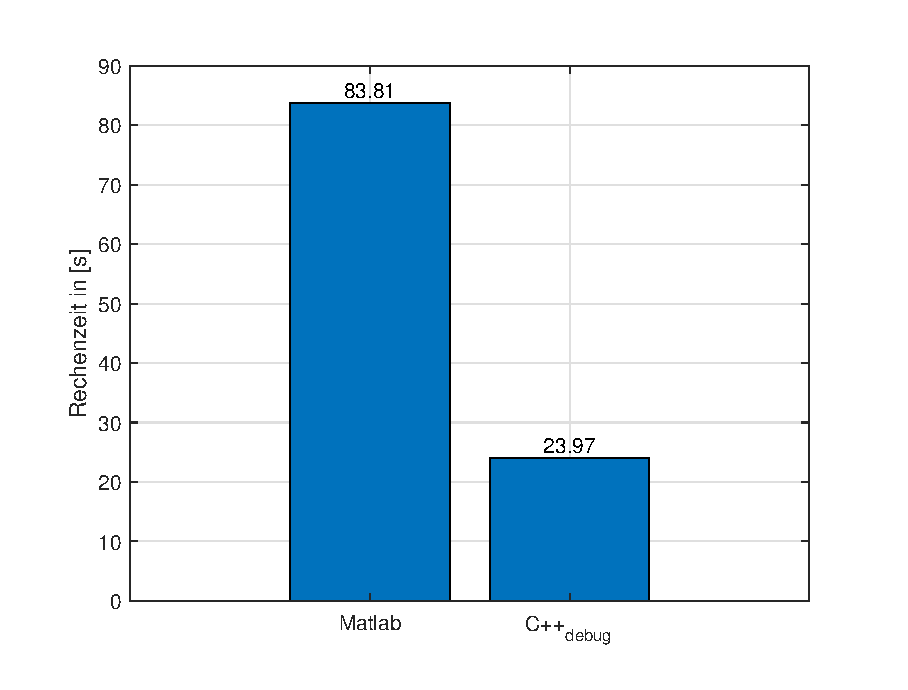
\includegraphics[width=0.6\linewidth]{Direktvergleich}
	\caption{Direktvergleich Matlab und C++}
	\label{fig:direktvergleich}
\end{figure}\noindent \\
Betrachtet man das Ergebnis von der quantitativen Seite und berechnet den relativen Rechenzeitunterschied ist das C++ Programm 71,4\% schneller als Matlab. Dieses Ergebnis ist weniger verwunderlich, da C++ das Programm in Maschinencode übersetzt. Matlab ist eine proprietäre Programmiersprache die auf dem jeweiligen Rechner interpretiert wird und kann dementsprechend die Ressourcen des Computers nicht voll ausnutzen.\\
Mit diesem Ergebnis wurde ein Ziel dieser Arbeit, die Rechenzeit zu reduzieren, erreicht.


\chapter{Optimierung der Simulation}
\label{ch:opt}
In der vorangegangen Kapiteln wurde die Umsetzung der Simulation erläutert und gezeigt, dass ein funktionsfähiges Framework validiert werden konnte. Im letzten Schritt dieser Ausarbeitung geht es um die Performance Optimierung hinsichtlich der Rechenzeit. Somit soll die Effizienz gesteigert und Schwachstellen im Code korrigiert werden. An dieser Stelle werden die Randbedingungen kurz erläutert, um gleiche Testbedingungen zu garantieren und um die Ressourcen des Rechners vollständig auszunutzen:
\begin{itemize}
	\item Um statistisch aussagekräftige Ergebnisse bezüglich der Rechenzeit zu erhalten werden 5 Läufe durchgeführt und am Schluss gemittelt.
	\item Hintergrundprozesse sollen vermieden werden.
	\item Der Rechner (Laptop) soll an einer Stromquelle angeschlossen sein. 
\end{itemize}
\section{Profiling}
Mithilfe des in Visual Studio integrierten Leistungsprofilers  wird das Laufzeitverhalten der Simulation untersucht. Somit sollen Problembereiche aufgezeigt werden, die kritisch hinsichtlich der Rechenzeit sind. In dieser Arbeit wird der Profiler genutzt, um die Anzahl der Aufrufe und Durchläufe von Funktionen festzustellen. Somit kann das Hauptaugenmerk auf Funktionen gerichtet werden, die durch ihre Aufrufe viel Zeit in Anspruch nehmen. In Tabelle \ref{tab:.profiler} werden besagte Funktionen mit ihrer jeweiligen CPU-Zeit aufgelistet. 
\begin{table}[h]
	\centering\begin{tabular}{llp{5cm}l}
	\textbf{Nr.} &	\textbf{Methode} & \textbf{Kurzbeschreibung} &\textbf{CPU-Zeit}\\
	1&	Trajectory6Dof::log6DofData() & Daten-Logging der einzelnen Module&50,79\% \\
	2&	updateAutopilot::updateStateController(...) & Zustandsregler & 22,62\% \\
	3&	LinearInterpolation::linearInterpolation2D(...) & Tabellen-Interpolation & 13,18\%
	\end{tabular}
\caption{Ergebnisse des Leistungsprofilers}
\label{tab:.profiler}
\end{table}\noindent\\
Es ist offensichtlich, dass das Erzeugen der Output-File den größten Einfluss auf die Gesamtrechenzeit hat. Im nächsten Schritt müssen mögliche Ursachen gefunden werden, die für die jeweiligen Funktionen die Rechenzeit beeinflussen. Im Anschluss muss eine Lösung für die Rechenzeit-Reduktion gefunden werden. In Tabelle \ref{tab:korrektur} werden die möglichen Ursachen und Lösungsansätze gegenüber gestellt.
\begin{table}[h]
	\centering\begin{tabular}{lp{6cm}p{4cm}}
		\textbf{Nr.} & \textbf{Ursachen} & \textbf{Lösungsansatz}\\
		1 & -nicht benötigte Daten werden geloggt & -Reduktion des Outputs \\
									  & -std::to\_string (25,5\%) & -alternative Methode finden (Benchmarking)\\
									  &&\\
		2 & Eigen::Library & alternative Bibliotheken \\	
									  &&\\
		3	& Index suche im Array & 	Suchmethoden anpassen		
	\end{tabular}
	\caption{Gegenüberstellung Ursachen und Lösungsansätze der Rechenzeit}
	\label{tab:korrektur}
\end{table}
\section{Code Optimierung}
Wie in Tabelle \ref{tab:korrektur} beschrieben, wurde unter Punkt 1 der Output der einzelnen Module reduziert. Zusätzlich wird im nächsten Abschnitt nach Alternativen für die \textit{std::to\_string} Methode gesucht. Da das Hauptaugenmerk auf der Überprüfung der Flugregelung steht, wurden Parameter vernachlässigt, die wenig Aussagekraft darüber besitzen.\\ Der Flugzustandsregler (Punkt 2) selbst beruht in großen Teilen auf linearer Algebra. In dieser Ausarbeitung wurde die lineare Algebra durch die Open Source Bibliothek \textit{eigen} realisiert. Eine Effizienzsteigerung wäre mithilfe einer alternativen Bibliothek denkbar, wurde aber nicht weiter betrachtet. Der Aufwand, sämtliche mathematischen Operationen in der Gesamtsimulation abzuändern wäre zu groß. Nach \cite{TuxFamily.2018} gibt es spezielle Einstellungen für Visual Studio, um die Performance der Bibliothek zu steigern, welche letztlich umgesetzt wurden. \\  Für die Interpolation (Punkt 3) werden Stützstellen benötigt. Diese Stützstellen zu finden ist mit großem Aufwand verbunden, da dass gesamte Array durchsucht werden muss. Es wurde versucht, diese Suche zu beschleunigen. Diese algorithmische Optimierung hat sich als äußerst komplex rausgestellt und konnte nicht gelöst werden. Das Ergebnis des ersten Teils der Optimierung ist in Abbildung \ref{fig:opt1} zu sehen.\newpage
\begin{figure}[h]
	\centering
	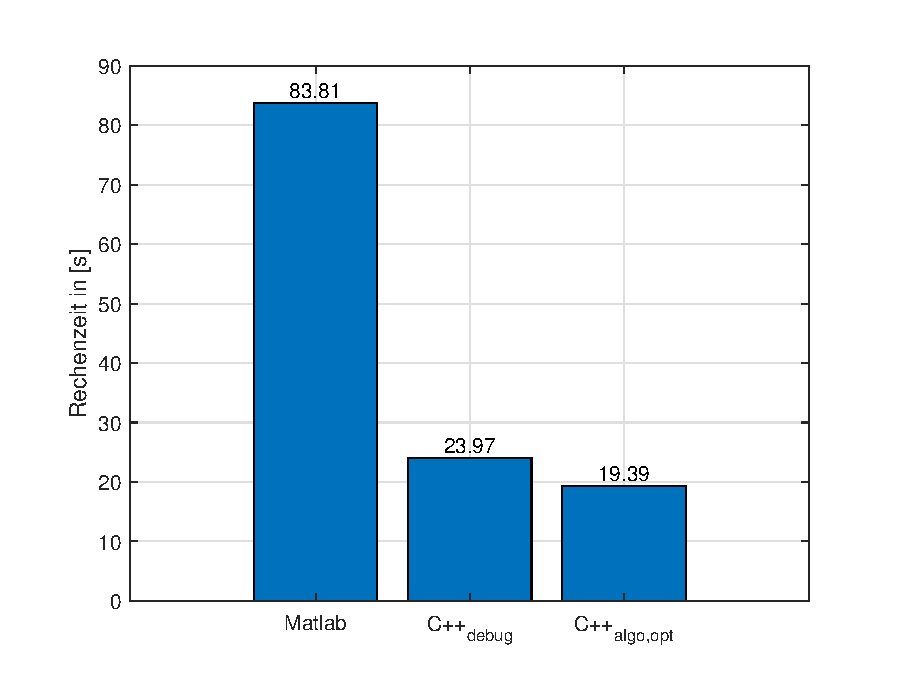
\includegraphics[width=0.6\linewidth]{opt1}
	\caption{Gegenüberstellung nach Code Optimierung Teil 1}
	\label{fig:opt1}
\end{figure}\noindent
Durch kleinere Maßnahmen im Code konnte die Rechenzeit nochmals um rund 4 Sekunden reduziert werden, was in etwa 19\% zum ursprünglichen C++ Code und 76,86\% zu Matlab schneller ist.
\subsection{Benchmarking String-Typumwandlung}
\label{sec:bench}
Wie in Tabelle \ref{tab:korrektur} angedeutet, beschäftigt sich dieser Abschnitt mit der Untersuchung von verschiedenen Möglichkeiten, die Typumwandlung in \textit{Strings} umzusetzen. Neben den Standardbibliotheken werden an dieser Stelle auch Open Source Bibliotheken hinzugezogen. Zum Einen wurden zwei Methoden der Boost-Bibliothek \cite{C++StandardsCommittees.2018} genutzt. Besagte Bibliothek wurde zur Produktivitätssteigerung in C++ erschaffen. Zum Anderen wurde die C++ String Toolkit Library (StrTk) von \cite{Partow.2018} genutzt. Dabei handelt es sich um eine Bibliothek, die speziell für den Umgang von Strings implementiert wurde. In Tabelle \ref{tab:benchmarking} werden die unterschiedlichen Methoden aufgelistet. 
\begin{table}[h]
	\centering\begin{tabular}{l}
		\textbf{Methode}  \\
			std::ostringstream \\
			sprintf\_s \\
			std::to\_string\\
			boost::lexical\_cast<std::string>(...)\\
			boost::str(boost::format("\%.4f") \% (value))\\
			strtk::type\_to\_string<double>(value)
			\end{tabular}
	\caption{Methoden für die Typumwandlung in \textit{String}}
\label{tab:benchmarking}
\end{table}\newpage
Das Ergebnis des Benchmarkings ist in Abbildung \ref{fig:benchmarking} zu sehen. In diesem Fall erwies sich die Methode sprintf\_s als sehr effizient.\\
\begin{figure}[h]
	\centering
	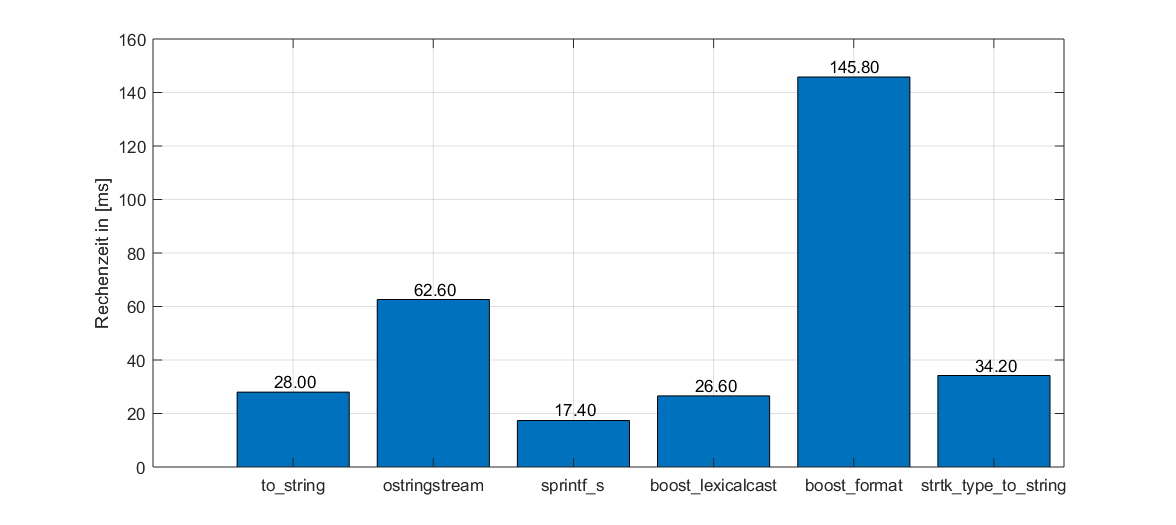
\includegraphics[width=0.8\linewidth]{benchmarking}
	\caption{Ergebnisse des Benchmarkings}
	\label{fig:benchmarking}
\end{figure}\noindent\\
 Die Methoden der Open Source Bibliotheken enttäuschen hingegen und werden aus diesem Grund in dieser Arbeit nicht weiter betrachtet. Aufgrund des Benchmarking-Ergebnisses wurde die std::to\_string Methode durch sprintf\_s ersetzt. Das Ergebnis der zweiten Code Optimierung ist in Abbildung \ref{fig:opt2} zu sehen.\\
\begin{figure}[h]
	\centering
	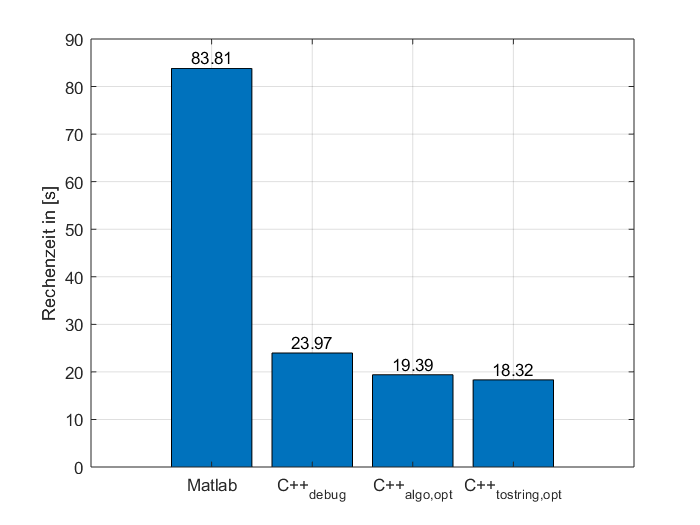
\includegraphics[width=0.6\linewidth]{opt2}
	\caption{Gegenüberstellung nach Code Optimierung Teil 2}
	\label{fig:opt2}
\end{figure}\noindent\\
Auch wenn die Rechenzeit sich nur minimal verbessert hat, so ist dies dennoch als gutes Ergebnis zu betrachten. Quantitativ ausgedrückt, hat sich die Rechenzeit gegenüber der ersten Optimierung konnten nochmals 5,5\% verbessert. Stand hier wurde die Rechenzeit gegenüber Matlab um 78,1\% verbessert.
\section{Parallelisierung und Vektorisierung}
Eine weitere Möglichkeit, neben der Code Optimierung, die Performance zu steigern ist die Zuhilfenahme von automatischer und gesteuerter Parallelisierung \cite{Kessler.Wintersemester201718}. Zusätzlich wurde auch noch der Einfluss von automatischer Vektorisierung untersucht. Die Ergebnisse der Parallelisierung sind auf den jeweiligen Rechner bezogen, wo diese durchgeführt wurde. Aus diesem Grund wird an dieser Stelle der Rechner, womit die Implementierung durchgeführt wurde, kurz aufgezeigt. Die grundlegenden Daten des Rechners sind in Tabelle \ref{tab:Rechnerdaten} zusammengefasst.
\begin{table}[h]
	\centering	\begin{tabular}{l p{10cm}}
		\textbf{Eigenschaft} & \textbf{Beschreibung/Wert}\\
		Betriebssystem & Windows 10\\
		Prozessor & Intel(R) Core(TM) i7-6600U CPU @ 2.60GHz 2.81GHz\\
		RAM & 8 GB\\
		Systemtyp & 64-Bit 
	\end{tabular}
	\caption{Rechnerdaten}
	\label{tab:Rechnerdaten}
\end{table}\\
Ausgangslage für die weitere Optimierung stellt das Ergebnis der  zweiten Code Optimierung aus Abschnitt \ref{sec:bench}.
\subsection{Automatische Parallelisierung und Vektorisierung}
Die automatische Parallelisierung und Vektorisierung kann schnell und einfach über Compiler-Flags durchgeführt werden. Der Compiler entscheidet selbstständig, ob er beispielsweise einen Abschnitt parallelisiert oder nicht. Die in dieser Arbeit genutzten Flags von Visual Studio werden in Tabelle \ref{tab:compilerflags} aufgezeigt. 
\begin{table}[h]
\centering	\begin{tabular}{ll}
		\textbf{Flag-Name} & \textbf{Verwendung}\\
		Qpar & automatische Parallelisierung\\
		arch & automatische Vektorisierung
	\end{tabular}
\caption{Compiler-Flags für automatische Parallelisierung und Vektorisierung}
\label{tab:compilerflags}
\end{table}\noindent\\
Die Flags werden sowohl einzeln als auch gemeinsam betrachtet. In Abbildung \ref{fig:compilerflags} sind die Ergebnisse dargestellt.\newpage
\begin{figure}[h]
	\centering
	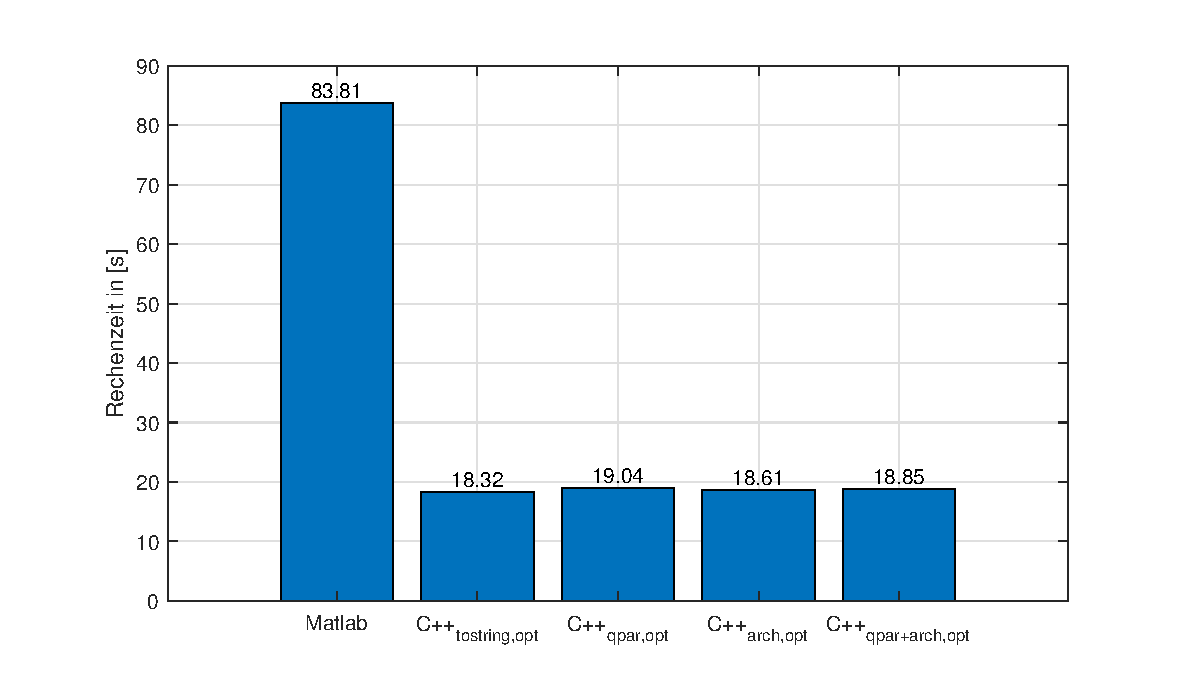
\includegraphics[width=0.7\linewidth]{compilerflags}
	\caption{Ergebnisse der automatischen Parallelisierung und Vektorisierung}
	\label{fig:compilerflags}
\end{figure}\noindent\\
Durch die automatische Parallelisierung und Vektorisierung wurde die Performance geringfügig schlechter. Dieses Ergebnis ist nach \cite{Kessler.Wintersemester201718} durchaus möglich. Aufgrund des fehlenden Performance-Gewinn, wird auf die Flags im Weiteren verzichtet. 
\subsection{Gesteuerte Parallelisierung}
Bei der gesteuerten Parallelisierung wird der Compiler durch Direktiven im Code angewiesen eine Parallelisierung durchzuführen. In dieser Ausarbeitung wurde der OpenMP Standard genutzt.\\
Es war leider nicht möglich, ein sinnvolles Ergebnis zu erzeugen. Grund hierfür liegt im Ablauf der Simulation selbst. Die Berechnung der Trajektorie findet lediglich in einer for-Schleife statt. Somit sind die Ergebnisse der direkt aufeinanderfolgenden Zeitschritte abhängig voneinander. Aus rein physikalischer Sicht ist es beispielsweise nicht möglich, dass ein Thread schon den nächsten Zeitschritt berechnet, bevor der vorangegangene Zeitschritt berechnet wurde. Somit wird auch die gesteuerte Parallelsierung nicht weiter betrachtet.\\



\chapter{Schlussbetrachtung}
\section{Diskussion des Gesamtergebnis}
Eines der Ziele, ein generisches Simulations-Framework für Flugzeuge in C++ zu implementieren wurde dadurch erreicht, dass sämtliche Parameter aus Input-Files eingelesen werden und die Methoden sehr allgemein gehalten wurden. Durch den modularen Aufbau können die einzelnen Module jederzeit um weitere Klassen erweitert werden. Die Simulation selber kann über ein Input-File gesteuert werden, womit unterschiedliche Modelle und Ausbaustufen ausgewählt und simuliert werden können, ohne dass der Nutzer den Code selbst verändern muss. In Kapitel \ref{ch:opt} wurde die Performance Optimierung der Simulation erläutert. Das Ziel, die Rechenzeit gegenüber Matlab  zu verbessern und im Nachgang weiter zu optimieren wurde erfüllt, wie in Abbildung \ref{fig:optergeb} zu sehen ist. 
\begin{figure}[h]
	\centering
	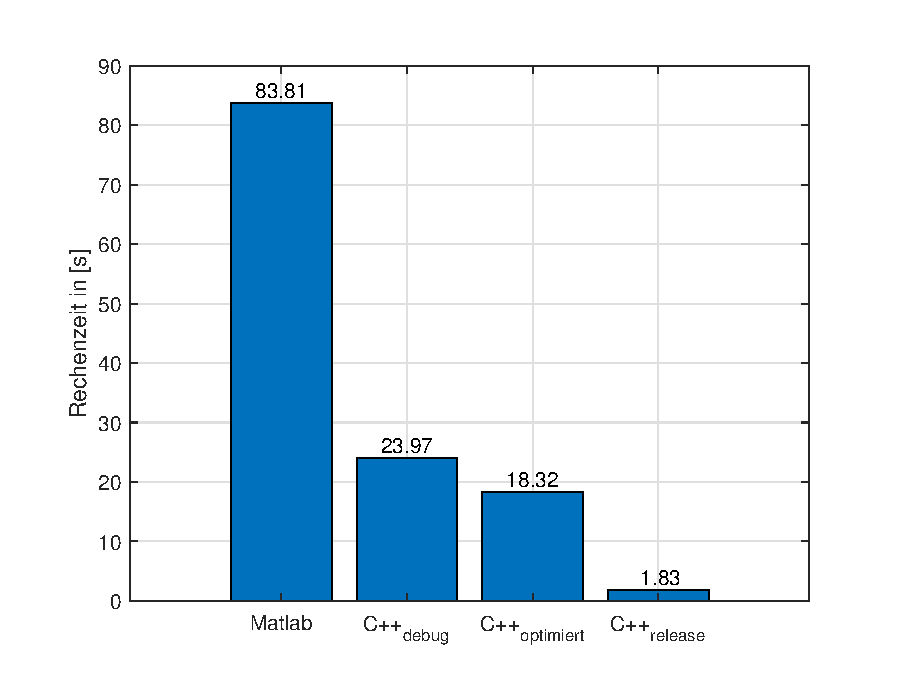
\includegraphics[width=0.7\linewidth]{untitled}
	\caption{Vergleich der Rechenzeiten}
	\label{fig:optergeb}
\end{figure}\noindent\\
Durch die Kompilierung als Release, konnte nochmals ein erheblicher Performancegewinn erzielt werden. Quantitative ergibt sich dadurch eine Rechenzeiteinsparung von 97,2\% gegenüber Matlab.
\section{Erweiterungsmöglichkeiten}
Das Simulationsframework kann aufgrund des modularen Aufbaus jederzeit um weitere Klassen ergänzt werden. Es wurde bereits erwähnt, dass die höchste Ausbaustufe derzeit noch keine Fehlermodelle der Subsysteme besitzt. Diese und auch andere Erweiterungen könnten in Zukunft implementiert werden. Derzeit werden die Unit- und Modultests nur manuell durchgeführt. Eine Automatisierung der Tests wäre denkbar. 
\section{Fazit}
Die in dieser Arbeit gesetzten Ziele wurde mit Erfolg erfüllt. Die Verwendung von Polymorphie wird als sehr effektiv angesehen, um ein Programm modular aufzubauen und um Code zu sparen. Zudem haben sich die in \cite{Kessler.Sommersemester2017}  und \cite{Kessler.Wintersemester201718} vorgestellten Tools zur effizienten Programmierung bewährt. Die zusätzlich Codedokumentation erwies sich als zusätzliche Last und fordert eine gewisses Maß an Selbstdisziplin. Durch die Durchführung von Unit- und Modultests, konnte die Funktion einiger Methoden nachgewiesen werden. Dennoch ist es sehr schwierig die Tests so zu definieren, um eine große Codeabdeckung zu gewährleisten. Der Leistungsprofiler ist sehr empfehlenswert, um Schwachstellen im Code zu erkennen und nachträglich algorithmisch zu optimieren. Die Möglichkeit der Parallelisierung konnte in dieser Ausarbeitung aufgrund des physikalischen Hintergrunds der Simulation nicht genutzt werden. Zusammenfassend lässt sich sagen, dass dem Nutzer eine funktionsfähige effiziente Simulationsumgebung für Flugzeuge zur Verfügung gestellt wird. 




%\printbibliography
\newpage
\bibliography{Quelle}

\end{document}